\begin{columns}[t]
	\begin{column} {0.42\textwidth}
		\begin{block}{\large Dataset Generation Tool}
			\centering
			\begin{itemize}
				\item The software tool for dataset generation is publicly released and can be found at \url{https://github.com/cmitash/physim-dataset-generator}
				\item It uses the {\tt Blender} python API for simulation and rendering.
				\item The repository also includes CAD models for 16 objects from {\it Amazon Picking Challenge 2016}.
				\item The camera parameters, choice of environment, and lighting options are provided as tunable parameters.
				\item The tool could be used to generate scenes with either bounding-box or pixel-wise class labels for objects.
			\end{itemize}
			\begin{columns}[t]
			\begin{column} {0.33\textwidth}
			\begin{figure}[h]
				\includegraphics[width=0.8\textwidth]{ex1}
				\caption{example image}
			\end{figure}
			\end{column}
			\begin{column} {0.33\textwidth}
			\begin{figure}[h]
				
\includegraphics[width=0.8\textwidth]{ex2}
				\caption{pixel-wise labeling}
			\end{figure}
			\end{column}
			\begin{column} {0.33\textwidth}
			\begin{figure}[h]
				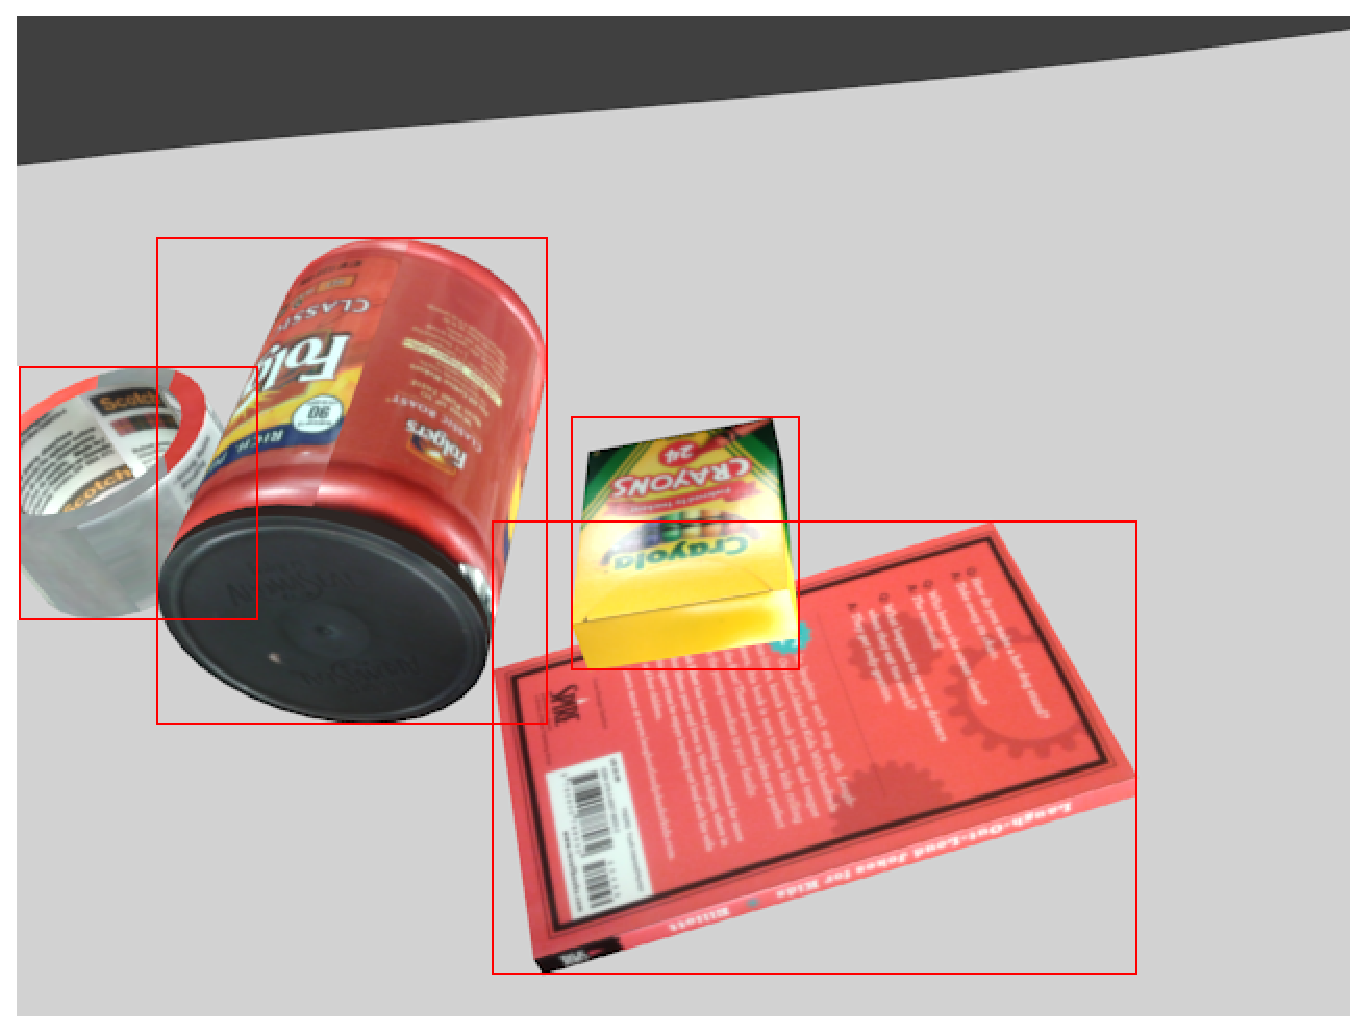
\includegraphics[width=0.8\textwidth]{ex3}
				\caption{bounding-box labeling}
			\end{figure}
			\end{column}
			\end{columns}
		\end{block}
	\end{column}

	\begin{column}{0.30\textwidth}
		\begin{block} {\large Evaluating Object Detection}
			\centering
			\begin{itemize}
				\item Evaluation is performed on {\tt Shelf \& Tote} benchmark dataset.
				 % released by Team MIT-Princeton participating in APC 2016. 
				% Reported result is detection success(\%) i.e Intersection-over-union $>$ 50\%
				\item {\tt Faster-RCNN} is trained using approximately 2000 physically-realistic scenes.The small number helps avoid overfitting with respect to texture and scene illumination.
			\end{itemize}
			\begin{figure}[h]
				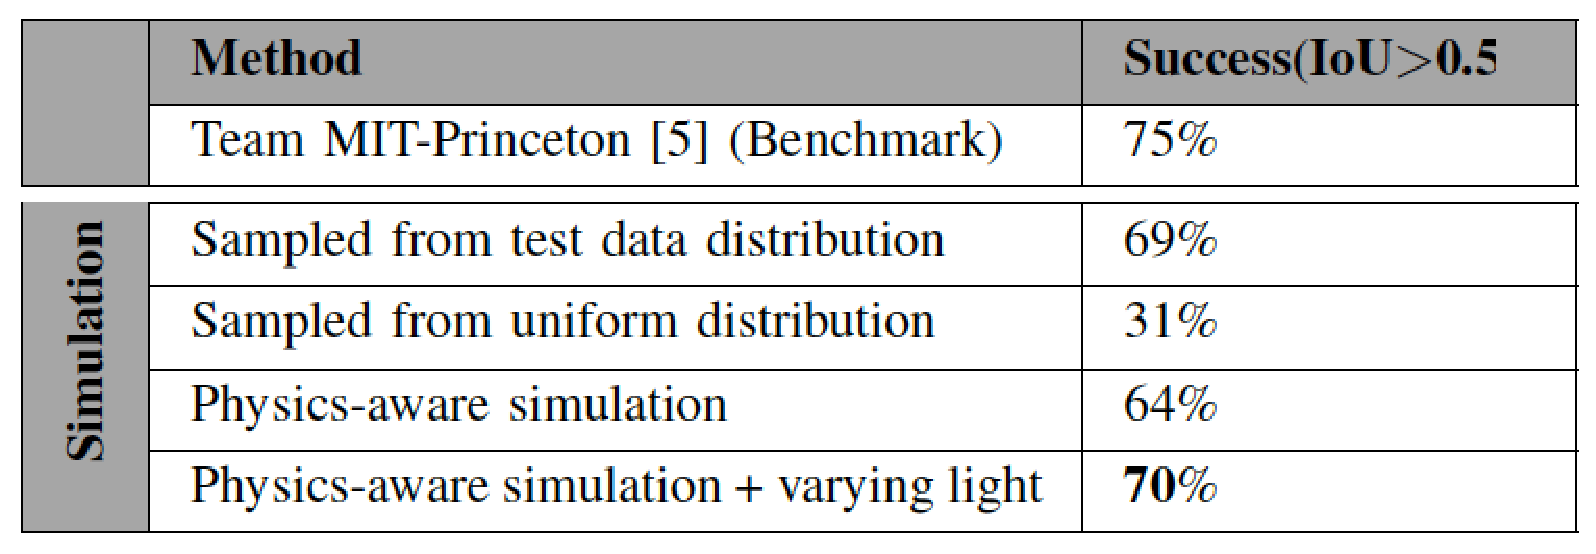
\includegraphics[width=0.9\textwidth]{detectRes}
			\end{figure}
			\vspace{-0.1in}
			\begin{figure}[h]
				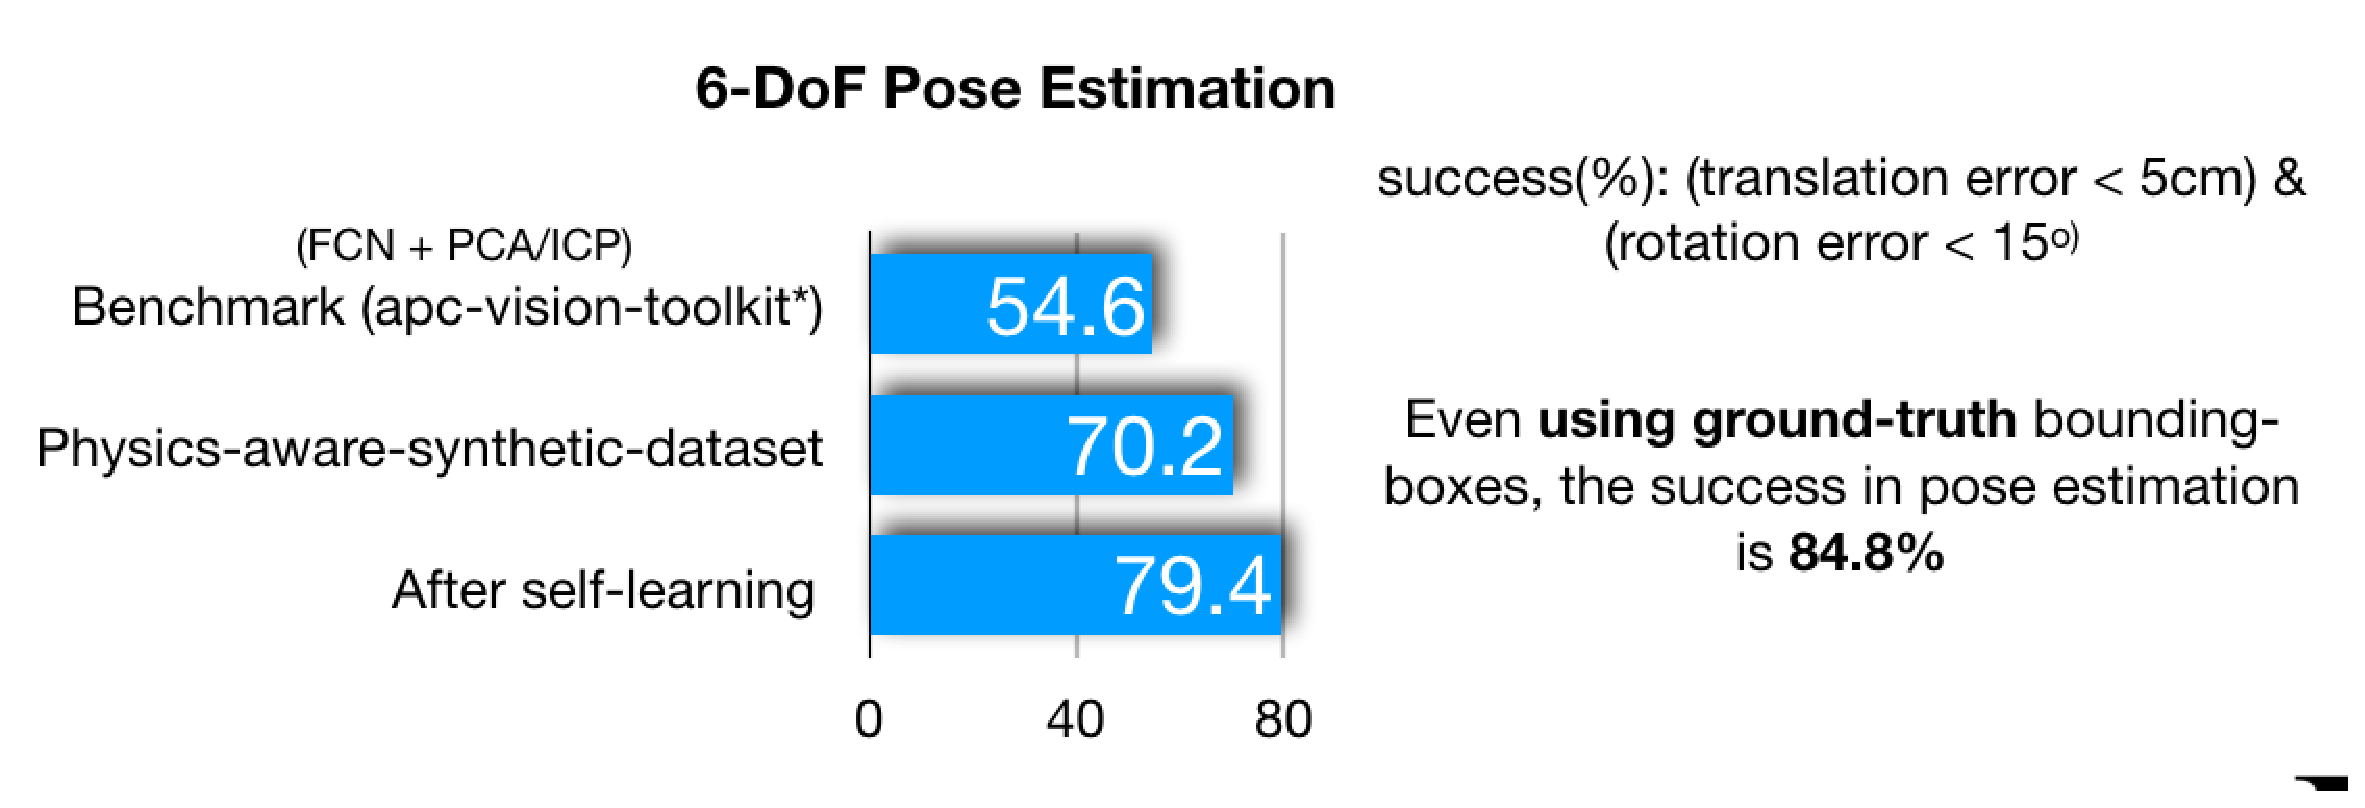
\includegraphics[width=0.9\textwidth]{eval_pose}
			\end{figure}
		\end{block}
	\end{column}
	\begin{column}{0.28\textwidth}
		\begin{block}{\large Motivation for MCTS}
			\centering
			\begin{itemize}
				\item Model-matching to individual object segments often result in pose estimates of objects that are physically inconsistent with other objects.
				\item Efficient search technique is required to search over the combination of individual pose hypotheses which best explains the observed scene.
			\end{itemize}
			\vspace{0.3in}
			\begin{columns}[t]
			\begin{column} {0.45\textwidth}
			\begin{figure}[h]
				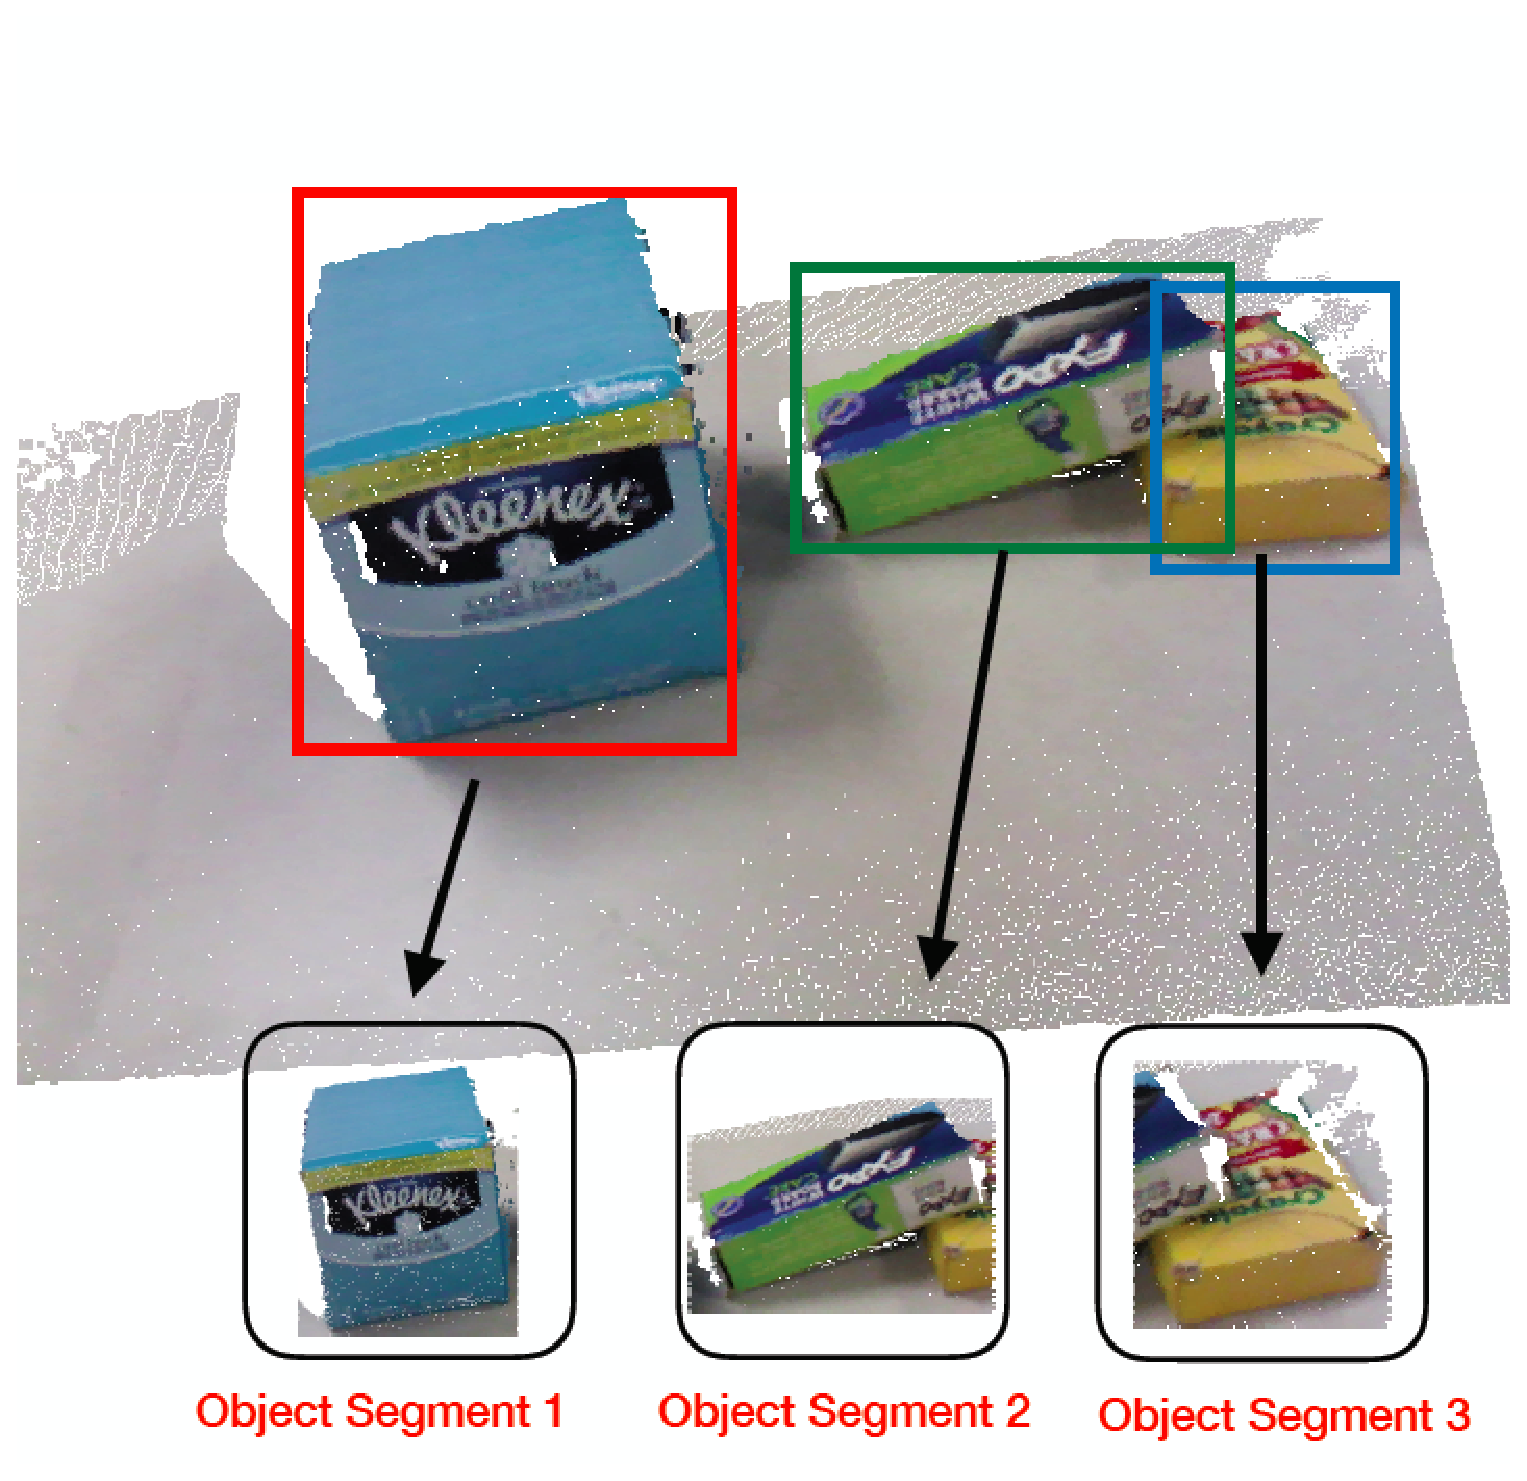
\includegraphics[width=0.75\textwidth]{obj_seg}
				\caption{Object segmentation with Faster-RCNN}
			\end{figure}
			\end{column}
			\begin{column} {0.45\textwidth}
			\begin{figure}[h]
				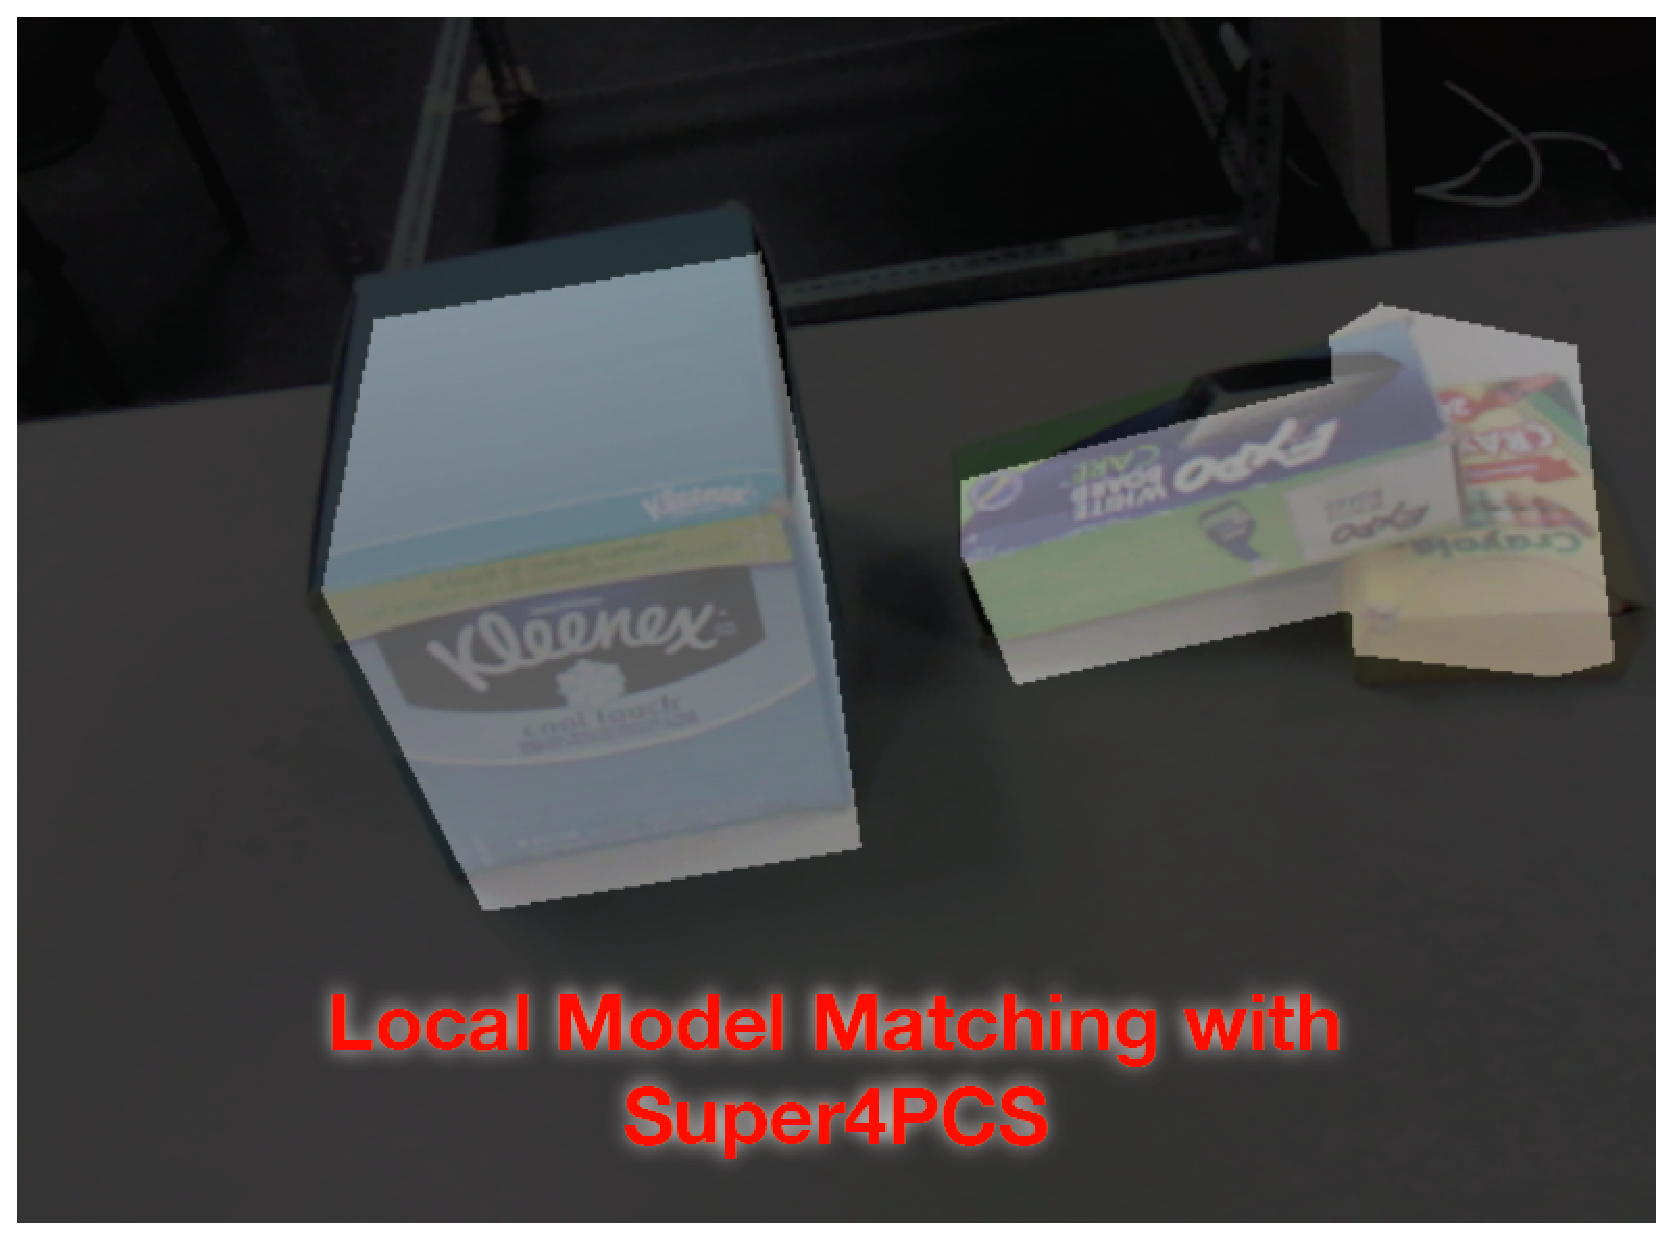
\includegraphics[width=0.9\textwidth]{local_match}
				\caption{Result of model-matching using Super4PCS}
			\end{figure}
			\end{column}
			\end{columns}
		\end{block}
	\end{column}
\end{columns}



